\begin{figure*}[t]
\centering
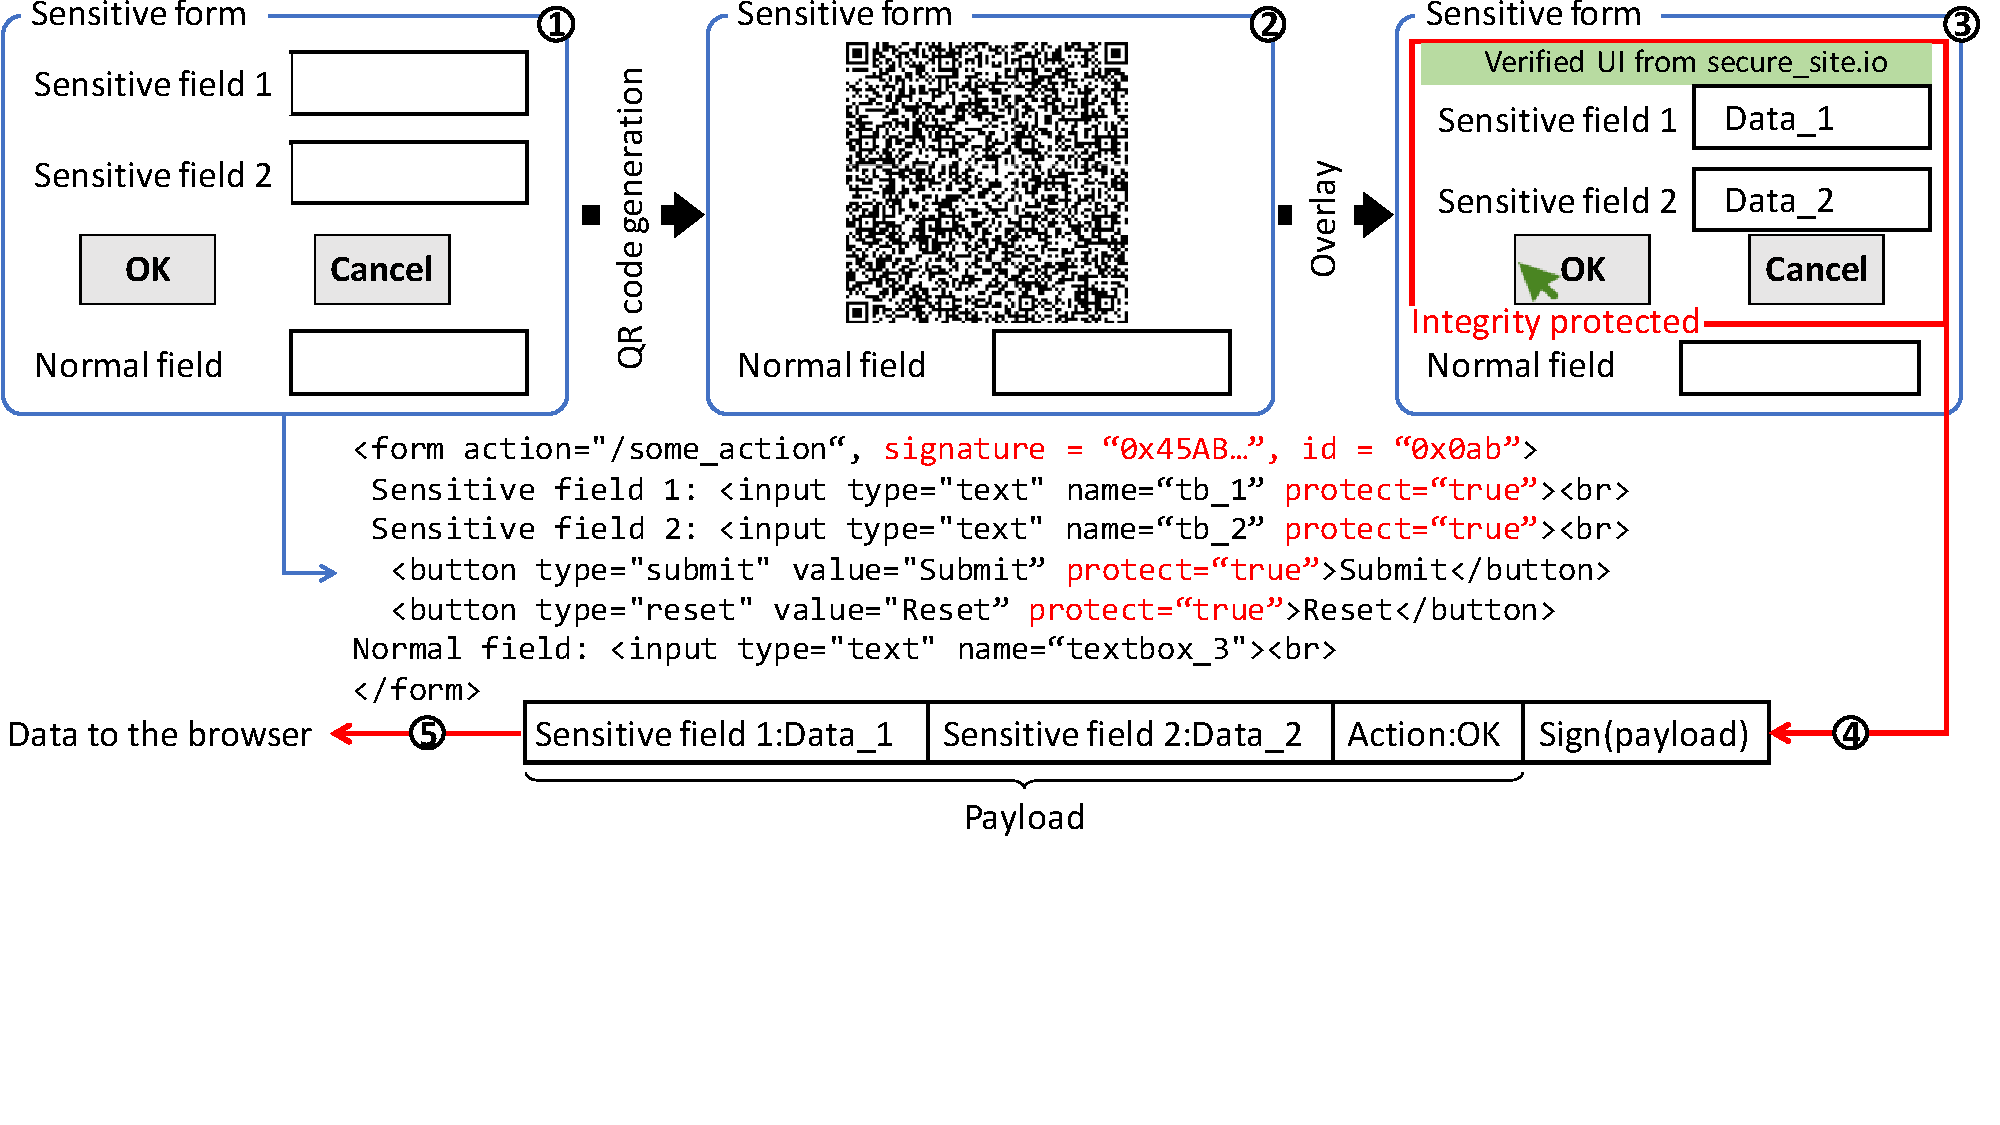
\includegraphics[trim={0 4.8cm 0 0}, clip, width=0.8\linewidth]{formTransform.pdf}
\caption{\textbf{Transformation of UI elements: HTML $\rightarrow$ encoded specification $\rightarrow$ \device generated UI overlay.} \one The actual webpage and the corresponding \html source shows the UI elements that requires integrity protection. \two These UI elements are transformed into an encoded UI specification (our \name prototype uses QR code that encodes a UI specification, e.g., Specification~\ref{snippet:UISpecification}) by the \name JS. The QR code. \three AThe QR code decoded and overlaid on the HDMI stream by the \device. \four Upon the user's action on the overlaid UI elements, the device signs all the input data. \five The \device sends these signed input data them to the remote server. Note that the intermediate QR code transformation (\two) is not visible by the user as it is decoded instantaneously by the device.}
\spacesave
\label{fig:transformation}
\end{figure*}

\section{\name for IO Integrity}
\label{sec:systemDesign}



\lstset{language=JSON, frame=tb, caption=\small{\textbf{Protected UI specification language.} The UI specification shows the JSON formatted UI specification that is generated from the \html source provided in the UI illustrated in Figure~\ref{fig:transformation}.}, label=snippet:UISpecification, firstnumber =1}

\begin{figure}[t]
\scriptsize
\begin{lstlisting}[mathescape=true]
{ "formId": "form1", "formName": "form1",
  "domain": "secure_site.io",
  "size": "400*400", "SAS": "5:LB",
  "ui": [{"id":"textbox_1", "type":"textbox", 
      "label":"Sensitive field 1",
    "text":"secret data 1",
    "RE":(A-Z)*.(A-Z)*},
    {"id":"textbox_2", "type":"textbox",
    "label":"Sensitive field2 ",
    "text":"secret data 2"},
    {"id":"b1", "type":"button",
    "label":"OK", "trigger":"true"},    
    {"id":"b2", "type":"button",
    "label":"Cancel", "trigger":"false"}],
  "signature": "0x45AB...", "id": "0x0ab.."}
\end{lstlisting}
\spacesave
\end{figure}

%In this section, we provide the technical details of \name for the integrity protection of IO devices. 
In this section, we provide the technical details of \name that guarantees the integrity of IO operations.


\subsection{\device Overlay of UI Elements}
\label{sec:systemDesign:transformation}

As we explained in the previous sections, both output and input integrity are necessary to be protected to achieve any of them. \name ensures output integrity by isolating a part of the display that cannot be observed or modified by the untrusted host. \device intercepts the HDMI frame from the host and injects a render of the sensitive UI on the screen. The overlay provides output integrity because it restrains the attacker from drawing on top of it to trick the user into providing incorrect inputs. 

To minimize the TCB, the \device does not run a browser, i.e., it can not interpret or render HTML, \js, etc. Instead, the \device comes with a small interpreter routine that is similar to render engines of browsers in functionality, but drastically smaller in size because it only renders a limited number of HTML5 UI elements according to their position, dimension, and label. The interpreter routine reads a given specification and renders the respective UI. The specification is a simple \emph{JSON} file that defines how the content of the overlay should be rendered, e.g., number of elements, order, types, and labels. \red{One strawman solution could be sending UI bitmap from the server to the \device and the \device could send back the mouse click and the corresponding location. \device could download these pre-generated form bitmaps from the server, and such solution would handle static forms, but not for dynamic forms. Downloading all possible form bitmaps would be prohibitively expensive.}

The process of rendering the overlay on the screen has two phases: (i) convert the existing sensitive form to specification, and (ii) specification to overlay.

\myparagraph{(i) Secure form $\rightarrow$ Specification} The W3C UI security policy~\cite{w3c_spec} recommends developers to annotate the security-critical UI elements of a page to protect them against malicious JS running on the browser. We use a similar technique by asking developers to manually annotate the sensitive elements in the HTML code (as \texttt{protect=``true''} attribute). Then For every request, the \name server-side component parses the HTML source, adds a random identifier (\texttt{id}) to the \texttt{form} element, signs it, add the \texttt{signature} to the \texttt{form} and then delivers it to the user's browser. The \texttt{id} serves as session identification to prevent the attacker from re-submitting an old input data from the user. On the client side, \name JS parses the tagged HTML source and produces a specification that can be interpreted by the \device.  An example of a specification is presented in~Specification~\ref{snippet:UISpecification}. In our implementation, the \name JS encodes the specification in a QR code. \red{We choose QR codes as it is one of the many robust was to encode data on a visual channel such as HDMI stream.} Figure~\ref{fig:transformation} shows the transformation between the step \one and \two. The step \two is processed by \device in the next phase and is not visible to the user.


%We further optimize this process that does not require to add the UI specifications into the HTML sources. The developers include small JavaScript code: \name JS to their sources. \name JS has the same functionally as the server side code that parses the HTML code and outputs the specification. Note the specification generation process is deterministic, hence, given identical HTML sources, both server and the \name \js generate identical UI specifications. Note that \name JS runs on the browser and is not trusted in our system model. We illustrate the method of UI transformation in Figure~\ref{fig:transformation}. 


\myparagraph{(ii) Specification $\rightarrow$ Overlay} \device performs the next phase, which starts with the detection of the encoded specification (QR-code) in the HDMI frames. Then the \device validates the signature, renders the overlay according to the specifications and presents it to the user.  The \device overlay is depicted in \three in Figure~\ref{fig:transformation}, which is the final UI shown to the user. Note that the user does not see the QR code as it gets decoded and overlaid by the \device on the fly.

\device uses the specification to determine the particular UI element that the user interacts with. When the user clicks on a text field, \device allows the user to type input to it. UI elements in the overlay take inputs only from input devices (mouse and keyboard). Therefore a malicious host cannot inject or modify any input of the user.

\subsection{Focusing User Attention}
\label{sec:systemDesign:userAttention}

In the previous section, we explain how \name provides output integrity for the overlay generated by the \device. However, the attacker can show fake information to the user on the untrusted part of the display space that may potentially influence her inputs. An advanced adversary could craft malicious directions and present to the user as part of the overlay.

To mitigate these attacks, we employ techniques that are proposed against similar threats in the context of browser-based security. The goal of these techniques is to focus user attention to the sensitive UI elements she is interacting with. Huang et al.~\cite{huang2012clickjacking} proposes two main techniques that are shown to be effective and can easily be adopted by the \device.  The first technique is called Lightbox, and it dims out non-overlaid part of the screen, which is generated by the untrusted host. The second technique consists of freezing display frames from the host when the user enters into the overlaid UI. This way, a malicious host cannot grab the user's attention by showing an animation or exploiting other tricks.
Lightbox offers more security guarantees because it blocks the untrusted screen completely, but is more intrusive to the user. While freezing is less intrusive but does not remove potential malicious information from the screen.
Lightbox mitigates the attacks presented above. The paper shows that the lightbox and freezing are effective in $98\%$ and $97\%$ of the time (baseline: $69\%$ effectiveness when no protection is provided) respectively, making them suitable candidates for \name. For more details of the user study, refer to Table 2 in~\cite{huang2012clickjacking}. We assume that similar result should be expected in \name due to the similarity of the application space (web applications). \device uses Lightbox as the default technique, but depending on the specific form, the developers can select the appropriate technique.

\red{Note that during the time the focusing mechanism (such as the LightBox) is active, the user can still interact with the UI elements and browser button outside the secure UI elements as the \device does not control those. Browser back button does not influence the state of the overlaid UI as long as it does not remove/change the QR code on the web page.}

\parasave
\myparagraph{\bfseries Automated activation} The technique to focus user attention (dimming out or freezing the non-overlaid part of the screen) is triggered automatically in specific situations: The user moves the mouse pointer over the overlaid UI, or the user starts typing into a sensitive UI element. 
%e.g., when the user moves her mouse pointer over the overlaid UI, or start moving the mouse after a brief pause (like 5 seconds). 
The advantage of the automated trigger is that the user does not need to remember to activate the mechanism. Hence the system is resilient from user habituation and does not require the user to actively monitor security indicators or perform specific actions. Note that the automated activation provides security to user IO data \emph{only} when integrity of the data is considered.

\subsection{Continuous Tracking of Mouse Pointer in the HDMI Frame}
\label{sec:systemDesign:analysis}


\begin{figure}[t]
\centering
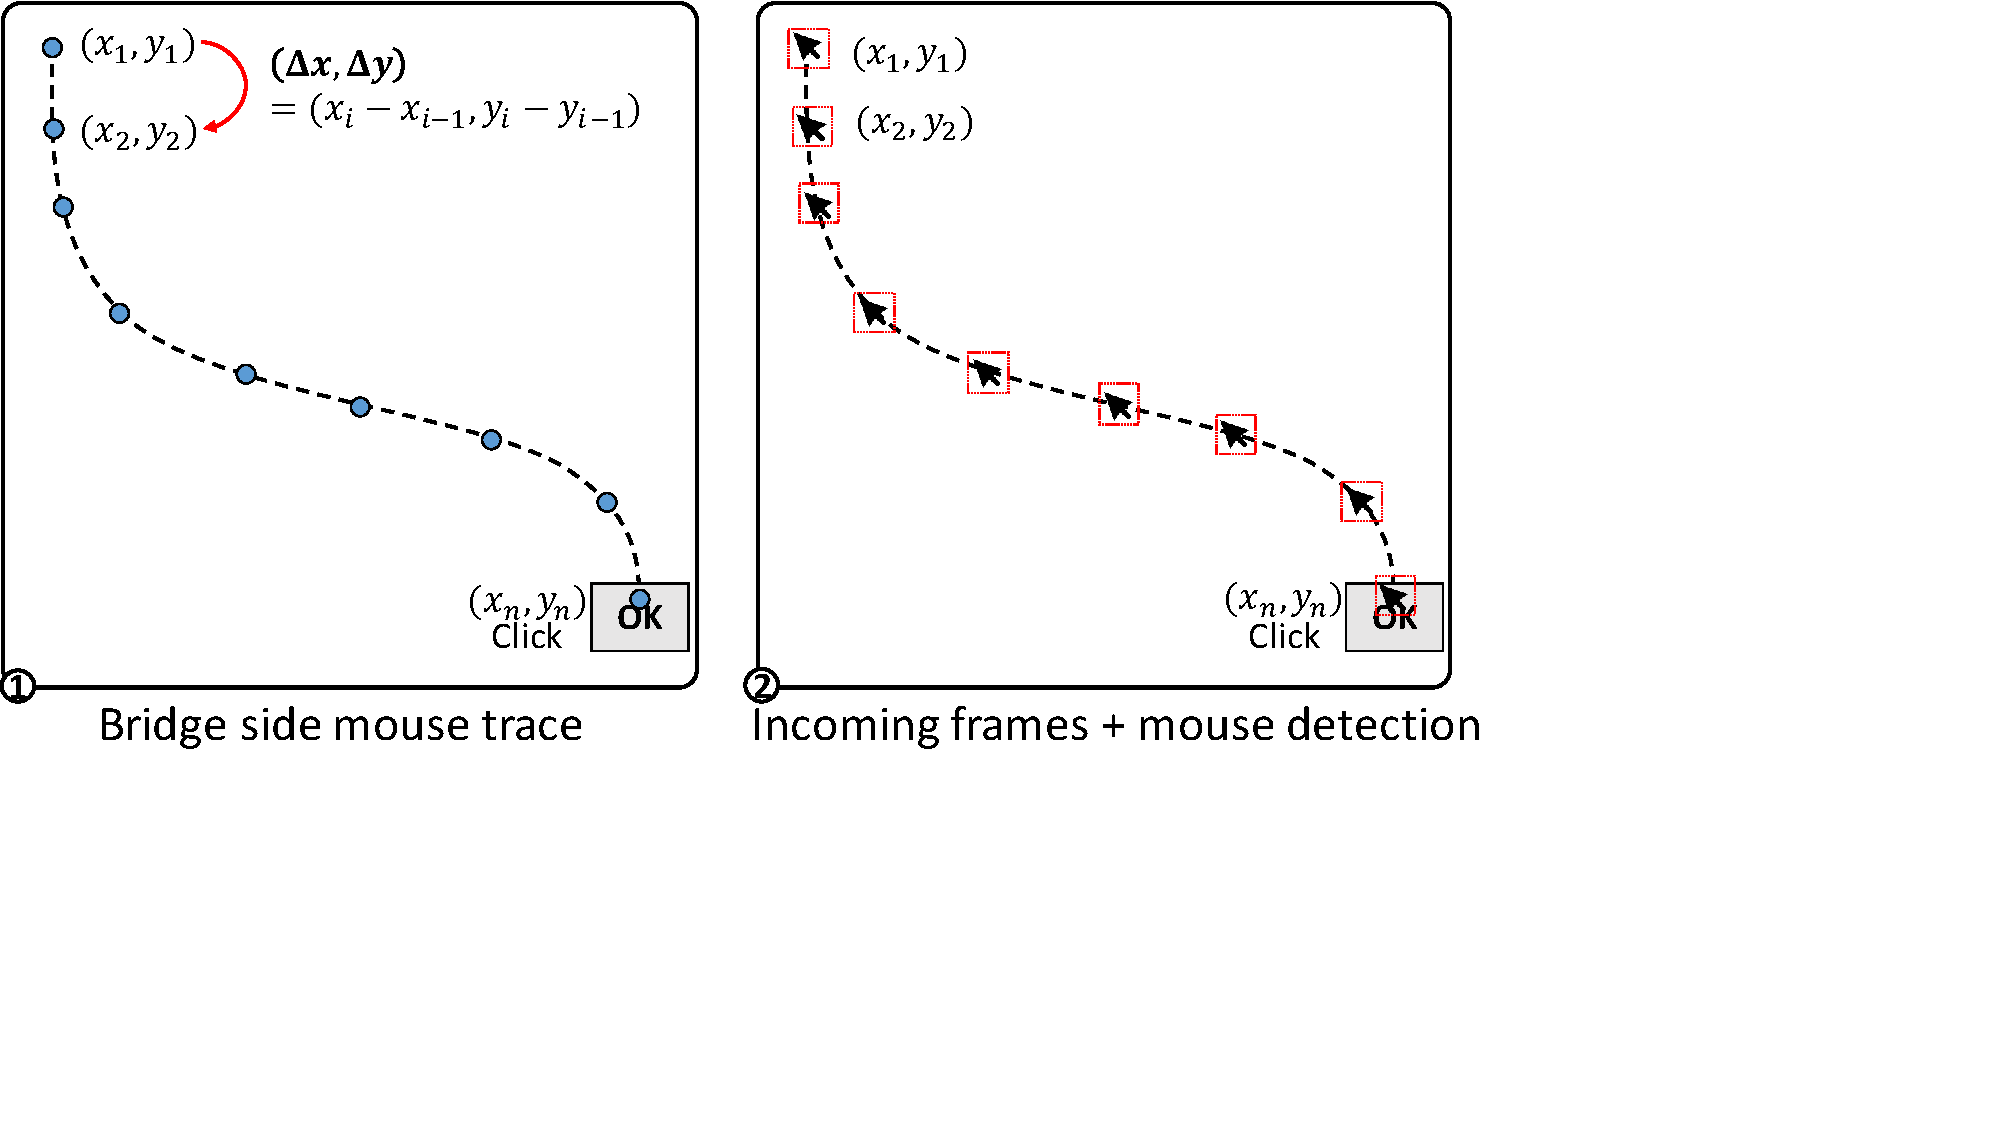
\includegraphics[trim={0 5.8cm 8cm 0}, clip, width=\linewidth]{mouseAnalysis.pdf}
\caption{\textbf{Pointer tracking.} \one The \device captures the raw mouse events ($\Delta x, \Delta y$) from the mouse that is attached to the \device. \two The \device captures the frames from the HDMI channel and checks into the designated pixel position $(x_i + \Delta x, y_i + \Delta y)$ if there exists a pointer. $t_1, t_2,\ldots t_n$ are the time instances when the \device receives the mouse data. $f_1, f_2,\ldots f_n$ are the corresponding HDMI frames that the \device intercepts.}
\spacesave
\label{fig:mouseAnalysis}
\centering
\end{figure}


The triggering of the focusing mechanism poses a challenging task to \name because the \device does not know the exact position of the mouse pointer. We cannot rely on the compromised host to communicate the pointer position reliably to \device. Furthermore, the host's pointer is not visible when the user interacts with the overlay rendered by the \device as the \device always draws on top of the HDMI frames of the host. 
%To address this issue, \name continuously tracks the host's mouse pointer from the HDMI frame (using shape detection) as it has access to both the HDMI channel and the raw mouse data.

\device could employ image analysis over the frame received from the host to learn the pointer position. However, we avoid this method because image analysis is time-consuming and vulnerable to adversarial images. In our approach, the \device intercepts mouse events and HDMI frames, so it can track the pointer based on mouse data and correlate it with the actual position in the HDMI frame (using shape detection in a small area). Then, the \device overlays a mouse pointer that is prominent and easy to follow by the user. 

A malicious host can still show a fake pointer to trick the user into following it, but when the focusing mechanism is active (the user interacting with sensitive elements), only the pointer overlaid by \device is visible. This way, the pointer tracking and the pointer overlay address three major challenges: i) both the \device and the user have the same sense of the pointer position, ii) \device knows precisely when to trigger the focusing mechanism, and iii) the user can interact with the overlaid UI seamlessly. 


\subsubsection{\bfseries Calibration}\label{sec:systemDesign:analysis:calibration} When the user connects the \device for the first time after booting up, the \device performs an automated calibration to find the pointer. The \device simulates the mouse and pushes the pointer to the top-right corner of the screen. Then the \device searches the pointer at this position in the HDMI frames
%If the \device is successful into finding the mouse pointer, 
and starts tracking the pointer afterward. Note, that at any point, if the \device loses track of the mouse pointer, the \emph{calibration} process is repeated the first moment the user visits a website that employs \name.
%user can recalibrate it by reinitializing the \device.

\subsubsection{\bfseries Pointer detection} The \device ensures pointer integrity by tracking the mouse movements using the raw data from the mouse and the HDMI frame.  Figure~\ref{fig:mouseAnalysis} illustrates the high-level idea: 

\begin{mylist}
\item[]\one Shows raw mouse data that notify the displacement events $(\Delta x, \Delta y)$ over $x$ and $y$ axis which are fired over time series $t_1,\ldots, t_n$. Note that the initial pointer position is known to the \device from calibration phase where $(x_0, y_0) = (0, 0)$.  
\item[]\two Shows the HDMI frames $f_1,\ldots f_n$ where the \device expects the mouse pointer to be found. For efficiency, the \device only scans a small portion of the HDMI frames ($200 \times 200$ square pixels) that is enough to cover a mouse pointer. Since the operating system can treat mouse movements slightly different according to their algorithm, this step serves to adjust the position difference.
%\device checks if there exists a mouse inside this square or not. \red{In case there exists a mouse cursor, the \device allows further user interactions; otherwise, it stops all the communications and shows an error on display.}
\end{mylist}


\subsubsection{\bfseries Overlay of the mouse pointer} The \device draws a mouse pointer overlay on top of the actual mouse pointer. The host mouse pointer is neither visible on top of the overlay nor it can interact with the \device's overlay. The overlaid mouse pointer is visible on top of the overlay, and it offers the same user experience as the host-rendered mouse pointer.


\subsubsection{\bfseries Coping with the disappearing pointer} Many OS offer a feature where the mouse pointer disappears from the screen when the user types in a text editor/browser. When the user moves her mouse, the cursor appears again at the same position where it disappeared in the first place. From the \device's perspective, it is hard to distinguish between this case and the attacker deliberately removing the mouse pointer from the screen. To handle this case, the \device listens to all the keyboard inputs -- the keyboard is also connected to the \device. Therefore, when the \device gets a keystroke event, it expects the cursor to disappear from the screen. Then, \device continues tracking the pointer from the moment that the mouse sends events  - this way, the \device ensures the consistency of the pointer position.  


\subsubsection{\bfseries Handling different mouse cursors} The \device is preloaded with template images of the mouse pointer for detection. For our \name prototype implementation, we use the default cursors provided by the Ubuntu OS. This allows the \device to identify the cursor when it changes on the screen, e.g., from pointer to a hand when the user hovers the pointer over a link on the browser. 

 
\subsubsection{\bfseries Handling mouse acceleration} The \device uses the default mouse acceleration parameters of \texttt{libinput} to cope with the pointer acceleration. As the \device emulates itself as a keyboard, at the time of initialization, the \device sends a command to the host to set the default acceleration. In case, the host changes the mouse acceleration; the \device will fail to detect the mouse in the HDMI stream. We consider this case as a denial of service.

\subsubsection{\bfseries Entering/exiting secure mode with keyboard} \red{In our implementation of \name, entering and exiting the secure mode could only be done by the mouse pointer. But similar could be done by the keyboard also. User could use the \texttt{TAB} button that selects the QR code on the browser. In the \name JS, we can define properties that triggers some changes (by changing the selection parameter) into the QR specification that signals the \device to enter/exit the secure UI.}

\begin{figure}[t]
\centering
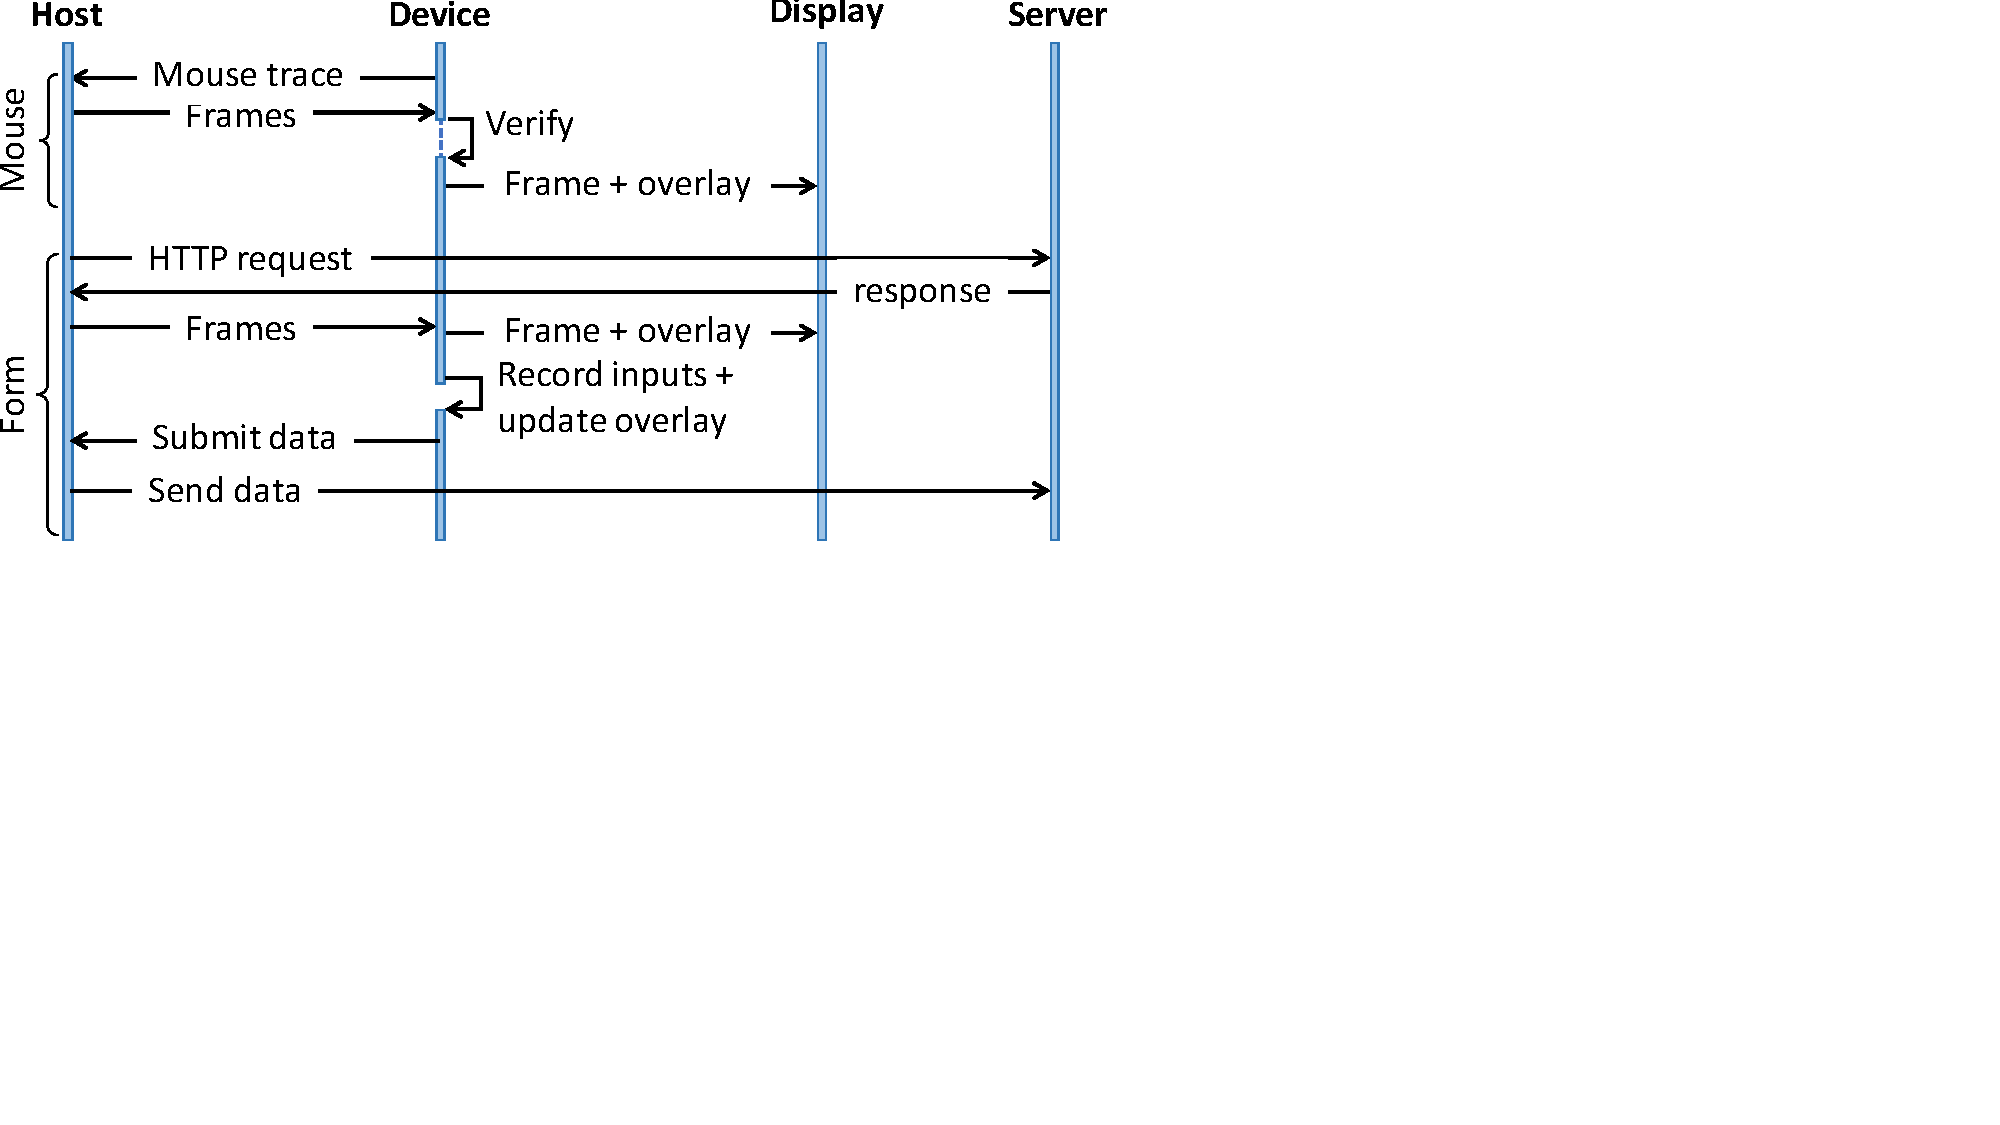
\includegraphics[trim={0 9.5cm 15cm 0}, clip, width=0.85\linewidth]{SequencDiagram.pdf}
\caption{\textbf{Flow of the \name main protocol.} The figure shows the sequence of events for two example scenarios: mouse movement and filling up a web-form.}
\spacesave
\label{fig:sequence}
\centering
\end{figure}


\subsection{Protected User Interaction}
\label{sec:systemDesign:commit}

When the user finishes providing her input via input devices (mouse and keyboard), the \device sends these values (with signature to ensure integrity) to the remote server. Sending these signed input values to the server requires an upstream channel from the \device to the server. 

\parasave
\myparagraph{Upstream channel}\label{sec:systemDesign:commit:upload} 
The data from the \device to the remote server is transmitted using the \name JavaScript snippet as a helper. 
%The \name JavaScript snippet uses a hidden text field to accept data coming from the \device. 
The \device emulates itself as a composite human interface device (HID) when it is connected to the host. The \device emulates keystrokes that transmit encoded data to the \name JavaScript snippet, which then forwards them to the remote server.

\parasave
\myparagraph{Sending input data} Figure~\ref{fig:sequence} depicts the user interactions in a sequence diagram. The user input transmission procedure is illustrated in Figure~\ref{fig:transformation}. This has two phases: \emph{record} and \emph{transmit} as described in the following:

\begin{mylist}
\item \textbf{Record.} After the UI elements are correctly overlaid on the screen, the users can interact with these UI elements. The user interaction with the overlaid UI element is no different than a standard UI. The UI specification encodes the behavior of all generated UI elements, making the \device aware of the semantics of the UI objects. E.g., when a user selects a text box and types on with her keyboard, the \device intercepts all keystrokes and renders the characters on the overlay.
When user enters input data in the rendered overlay UI elements (such as textbox, button, slider, radio button, etc.), the \device records that in a (key, value) pair where the key is the identifier of the UI element (\texttt{id} in Specification~\ref{snippet:UISpecification}) and the value is the user provided value. The \texttt{type} of the UI elements determines what information to record. For example, the \device records all keystrokes when a textbox is selected, the value corresponding to the position of the slider is recorded when the user interacts with a slider, etc. One example of the recording of the input data corresponding to the UI illustrated in Figure~\ref{fig:transformation} and Specification~\ref{snippet:UISpecification} is: 
\begin{align*}
Record = & (tb\_1, Data\_1);(tb\_2,Data\_2)
\end{align*}

\item \textbf{Transmit.} In the transmit phase, the \device waits for the user to select a UI element which has a \texttt{trigger} capability, e.g., a submit button on a web-form. A trigger element can change the state of the overlaid form, e.g., submit the data of the form to the remote server or reset it. More details are provided in the implementation of \name in Section~\ref{sec:prototype:impl:qr}. When the user clicks the \texttt{OK} button, the device signs $Record$ with its embedded private key. One such signed packet is also illustrated in Figure~\ref{fig:transformation}. The \device sends the signed packet to the remote server using the upstream channel.
\end{mylist} 

%\subsubsection{\bfseries Server-side verification} \label{sec:systemDesign:commit:verification}
Upon receiving the signed input data from the \device, the remote accepts the input if the signature verification is successful. Note, if an input field is annotated as \texttt{protect=``true''}, the server does not accept any input without the \device signature. This prevents the attacker-controlled host to submit data. 

\parasave
\myparagraph{Changing browser tabs or browsers}
The \device supports multiple browsing tabs across multiple browsers. The UI specification contains \texttt{formId} and \texttt{domain} that works as the unique identifier for a specific form served from a specific web server. The \device can maintain multiple parallel TLS connection to web servers. Depending on the observed \texttt{formId} and \texttt{domain} (refer to Specification~\ref{snippet:UISpecification}), the device retrieves the data that is entered by the user. This way even if the user switches tabs, the \device can still allow editing the forms across tabs.

\parasave
\myparagraph{Input validation} Input validation, i.e., checking the input against a recommended input policy (e.g., regular expression) is one of the most widely used JavaScript functionalities and it is a critical part of input integrity. The remote server sends the regular expression in the UI specification (\texttt{RE} in Specification~\ref{snippet:UISpecification}) that the \device uses to validate the user input.

%\myparagraph{Sequence of Events} In the previous Sections, we explain the basic components of \name. Here we summarize the overall flow of the system. The sequence diagram of \name is illustrated in Figure~\ref{fig:sequence} that shows snapshots of two example sequences: mouse movement and filling up a web-form.

\parasave
\myparagraph{Fallback for legacy clients} \name is backward-compatible with the clients who do not use the \device. This is achieved by the remote server by showing a QR code briefly on the screen when the user visits the \name-enabled webpage. The \device intercepted the QR code and sends a signal to the server about its presence. In the absence of the \device, the remote server does not send the \name JS to the host that acts as a communication channel between the \device and the remote server. Note, that the fallback mechanism is application-specific and the service provider could decide if the fallback is detrimental to security.